\documentclass[a4paper, 12pt]{book}


%packages
\usepackage{color} %color-package for text
\usepackage{mhchem} %nuclear notation package
\usepackage[english]{babel} %english language package
\usepackage{amsmath} %math-mode package
\usepackage{amssymb} %math-mode package
\usepackage{wasysym} %astrological symbols package
\usepackage{ifthen} %logical operations for new commands
\usepackage{graphicx}
\usepackage{placeins} %Use for floatbarrier-function
\usepackage{hyperref}
%commands
\newcommand{\comment}[1]{ {\color{red}#1} }
\newcommand{\importantcomment}[1]{ {\Huge \comment{#1}} }

%Packages and styles
\usepackage{natbib}
\bibliographystyle{../references/apj}

%Citation commands
\newcommand\araa{ARA\&A}
\newcommand\aaps{A\&AS}
\newcommand\apj{ApJ}
\newcommand\mycite[1]{{\footnotesize \it \citep{#1}}}

\newcommand{\isotope}[3]{{\footnotesize\ce{^{#3}_{#2}{#1}}}}
\newcommand{\eu}[1]{\isotope{Eu}{63}{#1}}
\newcommand{\re}[1]{\isotope{Re}{75}{#1}}
\newcommand{\os}[1]{\isotope{Os}{76}{#1}}
\renewcommand{\u}[1]{\isotope{U}{92}{#1}}
\newcommand{\pb}[1]{\isotope{Pb}{82}{#1}}
\renewcommand{\th}[1]{\isotope{Th}{90}{#1}}
\newcommand{\w}[1]{\isotope{W}{74}{#1}}

\newcommand{\sos}{Solar system}
\newcommand\betadecay{$\beta^-$-decay }
\newcommand\halflife{
  \ifmmode \tau_{\text{\tiny 1/2}}
  \else $\tau_{\text{\tiny 1/2}}$ \fi
}
\newcommand\msol{
  \ifmmode M_{\astrosun}
  \else $M_{\astrosun}$ \fi
}
\newcommand\omegamodel{\texttt{'Omega'}}
\newcommand\eris{\texttt{'Eris'}}
\newcommand\nsm{neutron star merger}


\begin{document}

\chapter{Compiling single sections at a time}
For writing purposes only.

\iffalse

\chapter{Theory Part II \comment{(need to rename)}}
\comment{Describe analytical models, numerical models (omega), simulations (eris) and that I compare the two latter}
\comment{Results from omega can be compared to hydrodynamical simulations like eris. Which are much more detialed and precise, but also more computationally expensive.}
\setlength{\figwidth}{0.8\linewidth}
\section{The \omegamodel\ model}
\label{sec:omega}
\omegamodel\ is a python code developed by Benoit C\^{o}t\'{e} and Christian Ritter\footnote{\url{https://nugrid.github.io/NuPyCEE/}}.
OMEGA stands for 'One-zone Model of the Evolution of Galaxies' and evolves the isotopic content of a galaxy\mycite{cote16a}.
The model is a one-zone model, which means that the entire galaxy is simplified to a single point.
A zero-space-dimensional galaxy model seems unrealistic, but it can be imagined as the mean value for a three-space-dimensional galaxy model.

%Define useful lengths
\newlength{\boxwidth}
\setlength{\boxwidth}{2cm}
\newlength{\boxheight}
\setlength{\boxheight}{1.5cm}
\newlength{\boxdepthx}
\setlength{\boxdepthx}{0.5\boxwidth}
\newlength{\boxdepthy}
\setlength{\boxdepthy}{0.5\boxheight}

%Define useful positions w/short-hand notation
%pos-position, b-bottom, t-top, l-left, r-right, f-front, d-distant
\newcommand\posbfl{(-\boxwidth,-\boxheight)}
\newcommand\posbfr{(\boxwidth,-\boxheight)}
\newcommand\posbdr{(\boxwidth+\boxdepthx,-\boxheight+\boxdepthy)}
\newcommand\posbdl{(-\boxwidth+\boxdepthx,-\boxheight+\boxdepthy)}
\newcommand\postfl{(-\boxwidth,\boxheight)}
\newcommand\postfr{(\boxwidth,\boxheight)}
\newcommand\postdr{(\boxwidth+\boxdepthx,\boxheight+\boxdepthy)}
\newcommand\postdl{(-\boxwidth+\boxdepthx,\boxheight+\boxdepthy)}

\begin{figure}
  \centering
  \begin{tikzpicture}
    %insert galaxy-image in center
    \node (galaxy) at (0.5\boxdepthx,0.5\boxdepthy) {\includegraphics[width=\boxwidth]{galaxy_thumbnail/galaxy.png}};
    %draw bottom plate
    \draw \posbfl -- \posbfr -- \posbdr -- \posbdl -- \posbfl;
    %draw top plate
    \draw \postfl -- \postfr -- \postdr -- \postdl -- \postfl;
    %draw vertical connectors
    \draw \posbfl -- \postfl;
    \draw \posbfr -- \postfr;
    \draw \posbdl -- \postdl;
    \draw \posbdr -- \postdr;
    %add inflow above box
    \draw[thick,->] (0,1.5\boxheight+\boxdepthy) -- (0,1.2\boxheight+\boxdepthy);
    %\draw (-0.5\boxdepthx,2\boxheight) -- (0,2\boxheight-0.5\boxdepthx) -- (0.5\boxdepthx,2\boxheight);
    %\draw (-0.25\boxdepthx,3\boxheight) -- (-0.25\boxdepthx,2\boxheight);
    %\draw (0.25\boxdepthx,3\boxheight) -- (0.25\boxdepthx,2\boxheight);
    \node at (0.6\boxwidth, 1.3\boxheight+\boxdepthy) {\small Primordial gas};
    %add outflow below box
    \draw[thick,->] (0,-1.2\boxheight) -- (0,-1.5\boxheight);
    %\draw (-0.5\boxdepthx,-2\boxheight) -- (0,-2\boxheight-0.5\boxdepthx) -- (0.5\boxdepthx,-2\boxheight);
    %\draw (-0.25\boxdepthx,-1\boxheight) -- (-0.25\boxdepthx,-2\boxheight);
    %\draw (0.25\boxdepthx,-1\boxheight) -- (0.25\boxdepthx,-2\boxheight);
    \node at (0.6\boxwidth, -1.3\boxheight) {\small Enriched gas};
  \end{tikzpicture}
  \caption{\label{tikz:galaxy-iobox}}
\end{figure}


In this work the \omegamodel\ code will be modified with a wrapper in order to explore various parameters related to nucleosynthesis.

\subsection{Process}
\label{sec:omega-process}
The \omegamodel\ model emulates the chemical evolution of a galaxy starting from the initial primordial gas. A simple stellar population is created by integrating the star formation rate over time.
The star formation rate is calculated either by using a constant star formation rate, the Kennicut-Schmidt law\mycitetwo{fuchs09}{and refernces therein}, or by using an input star formation rate and interpolate over those values.

The stellar populations represent a cluster of stars, with a total mass, initial mass distribution, and initial metallicity distribution.
The initial mass distributions are given as one of the standard distributions, Salpeter, Kroupa, Chabrier, or a power-law, all between some minimum and maximum mass limit (see figure \ref{fig:imf}.
The initial metallicity distribution is the relative mass distribution of isotopes heavier than \isotope{Li}{3}{7}, and the metallicity is the mass fraction of all isotopes heavier than \isotope{Li}{3}{7} combined.
\begin{figure}
  \centering
  \includegraphics[width=\textwidth]{img/various_initial_mass_functions.png}
  \caption{ \label{fig:various-imf}
    A simplified visualization of some of the common initial mass functions in the literature.
    \mycitetwo{cappellari12}{and references therein}, \mycite{salpeter55}, \mycite{kroupa01}, \mycite{chabrier03}, \mycite{miller79}. \\
    image-credit: By JohannesBuchner [CC BY-SA 4.0 (\url{https://creativecommons.org/licenses/by-sa/4.0})], from Wikimedia Commons
  }
\end{figure}


Stellar evolution codes calculate the amount of ejected material, for each isotope, for a star with a given initial metallicity and initial mass. These codes are used to create \textbf{yield tables} for certain kind of stars with different initial mass and metallicity.

In the simple stellar population assumed in the galactic chemical evolution model, these yield tables are used to calculate the chemical composition and mass of ejecta from each group of stars. The ejecta are disspersed back into the interstellar medium (gas of the galaxy model) at delay-times appropriate for each group of stellar mass.
E.g. For a given mass-bin the total mass in stars, number, and age of stars, with initial mass in that bin, are calculated using the total mass of the total stellar mass and mass function chosen. By choosing the yield tables closest in initial mass and initial metallicity the total ejecta composition is calculated and added to the interstellar medium at the age where those stars would have gone supernova.
The material that is not ejected is left as remnants and total mass and number of remnants are also added to the simulation at the time these stars would have gone supernova.

In \omegamodel\ the creation and treatment of simple stellar population is done by another python-program called \texttt{Sygma}.

The \omegamodel\ model is a \textit{one-zone} model, meaning that everything inside the box has been enriched from stellar lifecycles. Everything outside the box is untouched since ``it's creation'', and has the same composition as the material inside the box had to start with.
This composition is called the primordial composition (three parts hydrogen, one part helium and trace amounts of lithium and beryllium), and is derived from the big bang nucleosynthesis (see section\ref{sec:bbn}.
Flow of material can determine the chemical evolution of a galaxy. Enriched material can be ejected from the galaxy by supernova feedback, active galactic nucleus, stellar kick or similar, and non-enriched material can flow into the galaxy.
To describe the chemical evolution of a one-zone model one needs to know the total content of the galaxy (or box) and the distribution. In other words, how much of the total mass is stored as each isotope. Material with the same composition as the box is ejected from the box, and material with another composition falls into the box.

\comment{More on outflow/inflow}

\comment{Insert simple figure here}

\subsection{Uncertainty of parameters}
\comment{uncertainty of parameters and summary of article (cote16a)}

Galaxies consist of many different, widely varying, scales for both spatial and temporal resolution.
The galaxies themselves span hydrodynamical evolution on many kpcs and Gyrs, while their stars and supernovae span scales closer to seconds and meters.
The nuclear processes within stars span nanometer and millisecond timescales, even though stars can last for billion years(with short timescale bursts in between).
Neither analytical/numerical models nor simulations cannot cover all these scales at once, that is when subgrid methods are used. Stellar evolution simulations predict the fate and output from the life of a single star based on sinple input parameters and assumptions of the physical processes that governs the evolution. These solutions are then simplified and applied to more complex galaxy simulations.
Output ejecta from stars are ``looked up in a table'' and applied to the nearby interstellar medium.
All these methods and linked applications introduce some uncertainties and assumptions, both physical and numerical, and these uncertainties are inherited through all methods based on applications of these models. In order to probe how the uncertainties of selected parameters manifest through the resulting galaxy evolution, \mycite{cote16a} presents a simple one-zone, closed-box model of galaxy evolution, called \omegamodel.

%use \figwidth for width of image
\begin{figure}
  \centering
  \includegraphics[width=\figwidth]{img/uncertainty_diagram_cote16a_fig1.png}
  \caption[\mycitetwo{cote16a}{fig.1}]{ \label{img:uncertainty-diagram}
    Qualitative visualization of how uncertainties accumulate in galactic chemical evolution models.
    Experimental data on nuclear reaction rates are uncertain to some degree. The change in rate and uncertainty in stellar conditions are not well known.
    The conditions inside a star of a given mass and metallicity come from 1 dimensional hydrodynamical simulations.
    The combined result from nuclear reactions and hydrodynamical simulations give a stellar models.
    The stellar models are applied to a simple stellar population to account for all the billions of stars in galaxy.
    These stellar models are then applied to a large scale hydrodynamical simulation (like \eris), or a semianalytical galaxy model (like \omegamodel).
    All the steps make assumptions and add uncertainty to the grand total uncertainty that is difficult to map in completeness.

    Diagram is taken from \mycitetwo{cote16a}{fig.1}
  }
\end{figure}


\sygma creates the simplified stellar populations (mass function, total mass, lifetime distribution, initial metallicity).
\omegamodel\ combines several stellar populations to emulate a galaxy evolution.

Stellar yields are tables from stellar evolution simulations.
The tables used in \omegamodel are taken from, among other sources,  NuGrid\footnote{NuGrid collaboration: \href{http://www.astro.keele.ac.uk/nugrid/}{Homepage} \href{https://github.com/nugrid}{Github}} and include AGB stars between 1 and 7 \msol, massive stars between 12 and 25 \msol, all with metallicities at $Z = 0.02, 0.01, 0.006, 0.001, 0.0001$. These tables contain many isotopes between hydrogen and bismuth.

The stellar evolution was calculated with MESA\footnote{MESA is a modular, opensource code to evolve single star systems, and can do so from main sequence to white dwarf stage or core collapse stage. See \href{http://mesa.sourceforge.net}{Homepage} for further information}, post-processing was done with MPPNP \mycite{nugrid08mppnp}, the same nuclear reaction rates were used in all calculations, explosive nucleosynthesis was done with semi-analytical models. Yields are complemeted with SN1a yields from \mycite{sn1aivo13}, \mycite{sn1at03}, \mycite{sn1ai99}, \mycite{sn1at86} and population III yields from \mycite{pop3hw10} (other sources are available from the literature, but these are the focus of the chemical evolution of this thesis. Sources for neutron star mergers will be discussed later).

The probability distribution functions for the input parameters are created from values and uncertainties in the literature.
Methodologically there are, for each input parameter, gathered a list of literature values and uncertainties.
The errors are considered gaussian in nature and distributions are created thereafter,
all the distributions are then averaged to a single distribution.
Then a single gaussian is fitted atop the ``average of gaussians from the literature'',
and the median and standard deviation from
the final fit is used as value and uncertainty for the input parameter in question.

%insert images from cote16a to summarize the parameter-method
\setlength{\subfigwidth}{\linewidth}
\begin{figure}
  \centering
  \includegraphics[width=\subfigwidth]{img/parameter_pdfs_cote16a_fig2.png}
  \includegraphics[width=\subfigwidth]{img/parameter_table_cote16a_table7.png}
  \caption{\label{fig:cote16-input-param}
    How the input parameters were determined from multiple sources in the literature. Values and standard deviations averaged to a probaiblity distribution, and then fitted to a single gaussian distribution. Images from \mycitetwo{cote16a}{figure 2 and table 7}.
  }
\end{figure}

\mycite{cote16a} sampled a set calculations, for each parameter in figure \ref{fig:cote16-input-param} a series of 300 calculations were made with a random sampling of the input parameter for the gaussian uncertainty distribution.
A set of 700 calculations were made were all the input parameters were all the input parameters were randomly drawn from their respective gaussian distributions. An additional 300 calculations were made with the final gas-mass and final stellar mass both drawn randomly from their respective gausssian distributions.

Spectroscopic abundance of metals are measured in [X/Y] where X is the metal in question and Y is the reference metal, either plotted against metallicity, [Y/H], or galactic time, Gyr.

The main conclusions are summarized as follows:
\begin{enumerate}
\item{
  The overall uncertainty of spectroscopic metals between 0 and 0.6 dex when plotted against metallicity, but the uncertainty is higher when considered against galactic time.}
\item{
  \begin{itemize}
  \item{Ratio of final mass of gas to final mass of stars affect the uncertianty for early times ([Fe/H] $\lesssim$ -2) since more gas means more hydrogen, while more stars means more iron-production. Since metals are also produced in stars, the ratio does not affect [X/fe] much.}
  \item{Number of type 1a supernovae and their delay time distribution affect the uncertainty of spectroscopic metals at later times([Fe/H] $\gtrsim$ -1.5 $\rightarrow$ t $\gtrsim$ 150Myr), when the delay-time has allowed for type 1a supernovae to occur. Type 1a supernovae add mostly iron to the interstellar medium, while not producing much of metals produced by AGB stars and massive stars. This means that the uncertainty of [X/Fe] will be greatly affected by uncertianties in type 1a supernovae.}
  \item{The high mass slope of the initial mass function, $\alpha$, determines the ratio of massive stars to low-mass stars at all times. Massive stars die quickly and distributed much enriched material into the interstellar medium. Therefor the uncertainty of the slope will always be prevailent in the uncertainty of spectroscopic metals.}
  \item{Uncertainties in the mass ranges of the initial mass function does not affect uncertainties of the spectroscopic abundances much.}
  \end{itemize}
}
\item{
  Uncertainties in the slope of the initial mass function, $\alpha$, and the number of type 1a supernovae affect the uncertainties in the spectroscopic abundances.
  When plotted against metallicity ([Fe/H]) the uncertainty is greatest when the considered metal and the reference metal is not from the same source.
}
\item{
  The characteristics seen from spectroscopic abundance against metallicity is shared regardless of the introduced uncertainties.
  The introduced uncertainties amplify the characterstic shapes, but do not change them. ``Such features are mainly caused by the choice of stellar yields and the type of galaxy considered.''\mycitetwo{cote16a}{p.18}
}
\end{enumerate}

%use \figwidth for width of figure
  \centering
  \includegraphics[width=\figwidth]{img/spectroscopic_uncertainties_cote16a_fig6.png}
  \caption[\mycitetwo{cote16a}{fig.6}]{
    \label{img:spectroscopic-uncertainty}
    Spectroscopic abundance of 16 metals relative to iron, considering uncertainties of all parameters (upper bound, lower bound and high mass slope of initial mass function, stellar and gas mass today, number of type 1a supernovae and the slope of the type 1a supernova delay-time distribution).

    Plots and figures are taken from \mycitetwo{cote16a}{fig.6}
  }

%use \figwidth for width of figure

\begin{figure}
  \centering
  \includegraphics[width=\figwidth]{img/age_uncertainties_cote16a_fig11.png}
  \caption[\mycitetwo{cote16a}{fig.6}]{
    \label{img:age-uncertainty}
    Uncertainty of spectroscopic abundance of 16 metals relative to iron, considering uncertainties of all parameters (upper bound, lower bound and high mass slope of initial mass function, stellar and gas mass today, number of type 1a supernovae and the slope of the type 1a supernova delay-time distribution).

    Uncertainties relative to mean shown as a function of galactic age.

    Plots and figures are taken from \mycitetwo{cote16a}{fig.6}
  }
\end{figure}


\FloatBarrier

\subsection{Relevant parameters}
\label{sec:omega-parameters}
\omegamodel\ has many input parameters, both numerical and physical in nature, to guide the evolution of the galaxy. A physical input parameters are model parameters, while a numerical parameter decides on which calculations to choose from and where to get data. E.g initial gas of galaxy is considered physical, while the boolean switch to turn on neutron star mergers are considered numerical

This section will describe the most relevant ones in order of appearance in the program.

\begin{description}
\item[galaxy]
  This string option chooses predefined parameters to best match a certain galaxy on record.
  The relevant options are:
  \begin{description}
  \item[None] No parameters determined.
  \item[milky\_way\_cte] Set present dark matter mass to $10^{12} \msol$ and present stellar mass to $5\times10^{10} \msol$, and use a constant star formation rate of $1 \frac{\msol}{yr}$
  \item[milky\_way] Set present dark matter mass to $10^{12} \msol$ and present stellar mass to $5\times10^{10} \msol$, and use the star formation rate from \mycite{sfrcmr01}
  \end{description}
\item[in\_out\_control] Boolean switch to turn on or off inflow and outflow.
\item[outflow\_rate] \comment{remove this?} Constant outflow rate in $\frac{\msol}{yr}$. Enriched gas from the interstellar medium is removed from the galaxy.
\item[inflow\_rate] Constant inflow rate in $\frac{\msol}{yr}$. Gas with primordial composition \comment{(reference to BBN?)} flows into the galaxy.
\item[mass\_loading] Fraction of solar masses ejected per solar mass created as star. A different way of calculating outflow based on star formation rate.
\item[imf\_type] Which form to use for the initial mass function\comment{explain this somewhere}. 
\item[alphaimf] Slope of lognormal initial mass function. 
\item[sn1a\_rate] This string option chooses which distribution to calculate the rate of type 1a supernovaefrom.
  Options are powerlaw, gaussian, and exponential distribution.
  \begin{description}
  \item[beta\_pow] Set the power of the power law distribution if 'sn1a\_rate' is "power\_law" 
  \item[gauss\_dtd] Set the mean and standard deviation of the gaussian distribution if 'sn1a\_rate' is "gauss" 
  \item[exp\_dtd] Set the e-folding time of the exponential distribution if 'sn1a\_rate' is "exp"
  \end{description}
\item[dt] Length of first timestep (in yrs)
\item[special\_timesteps] Number of logarithmic timesteps
\item[tend] Final point in time (in yrs)
\item[mgal] Initial mass of gas (if not calculated by other means), defaults to $10^{10} \msol$
\item[transitionmass=8]
  Mass-limit that separates the AGB stars from the massive stars\comment{explain these stars somewhere}.
  Defaults to $8\msol$
\item[nb\_nsm\_per\_m] Set the number of neutron star mergers per solar mass formed as stars.
\item[t\_nsm\_coal] Set the time after which all neutron stars collide/merge
\item[table] path to yield table for AGB and massive stars.
\item[sn1a\_on] Boolean switch that turn on or off the use of type 1a supernovae.
\item[nsm\_dtd\_power] Set the powerlaw distribution of the neutron star merger delay-time distribution \comment{explain this somewhere}.
\item[sn1a\_table] Yield table for type 1a supernovae
\item[ns\_merger\_on] Boolean switch to turn on or off binary neutron star mergers
\item[f\_merger] Fraction of binary systems that eventually merge. All systems are considered binary. This is instead of 'nb\_nsm\_per\_m'
\item[m\_ej\_nsm] solar masses ejected per neutron star merger.
\item[nsmerger\_table] Yield table of binary neutron star mergers
\item[bhns\_merger\_on] Boolean switch to turn on or off black hole neutron star mergers
\item[pop3\_table] Yield tables for population III stars
\item[imf\_bdys\_pop3] The boundaries of the initial mass function of population III stars.
\item[nb\_1a\_per\_m] The number of type 1a supernovae per solar mass formed.
  Used to calculate the number of type 1a supernovae from star formation rate.
\item[popIII\_on] Boolean switch that turn on or off the use of Population III stars
\item[out\_follows\_E\_rate] Adds a time-delay to outflow with mass\_loading such that outflow follows supernova rate.
\item[sfh\_array] Two one-dimensional arrays, time and star formation rate, that \omegamodel will interpolate over in order to find the star formation rate at a given time.
\end{description}

%Add reference to Guedes 2011, shen 2015

%What is so fucking special about this thing?!?!?!?!
%how is gasoline used?!?!

\section{\eris simulation}

'Eris' is a N-body/smooth particle hydrodynamics simulation of a
galaxy forming in $\Lambda$CDM cosmology.
The simulation consist of dark matter particles and baryonic gas
particles. Star particles are created when the number density
passes 5 atoms cm$^-3$. Feedback from an active galactic nucleus
is neglected, but supernova-feeback is considered along with
cosmic UV background and radiative cooling.

Some properties of the simulated galaxy:
\begin{itemize}
\item{rotaional disk with scale length $R_d=2.5kpc$}
\item{``gentle'' rotation curve with circular velocities at 2.2
  scale lengths}
\item{i-band (infrared wavelength 806 nm, bandwidth 149 nm)
  bulge-to-disk-ratio of $B/D=0.35$}
\item{baryonic mass fraction inside halo is 30\% lower then
  cosmic average}
\item{thin disk with typical HI-stellar mass-ratio}
\item{disk is forming stars in $\Sigma_{sfr}-\Sigma_{HI}$ plane}
\item{disk falls on photometric Tully-Fisher relation and
  stellar mass - halo virial mass relation}
\item{structural properties, mass budget, and scaling relations between mass and luminosity matches several observational constraints}
\end{itemize}

In galactic simulations there is an ``angular momentum problem''. This refers to baryonic components having much less rotaional spin in simulations than real observations. This failure was believed to arise from friction moving angular momentum from sub-structures to outer halo when these sub-structures merge causing the cold clumps of gas to fall to the center.
In newer times this problem have been attempted solved with energy injected from supernovae, meaning evolving stars from the gas content to decrease the effect of cooling and removing angular moment from the center of the galaxy.
Star formation in the disk comes from inflow of cold baryonic gas that was never shock heated to virial temperature.
INSERT S0...-GALAXY-SHEET.
%link thesis/img/HubbleTuningFork.jpg

Yet the simulated galaxies have more centered baryon components and reproduce only S0 and Sa type galaxies. With two major exceptions there are no simulations of type Sb and Sc, one exception with low star formation and another with low mass.

This paper presents a realistic simulation of a Milky Way type galaxy using a new smotth particle hydrodynamic cosmological simulation. It includes radiative cooling, cosmic UV heating, supernova feedback, and high-density star formation requirement(which is believed to be a key ingridient.

The high threshold for star formation is important to create non-centered galaxies

%r-process post-production with Shen 2015
In Shen 15 \comment{(insert proper citation)} the simulation data from 'Eris' is post-processed to include, not only oxygen adn iron, but also europium from neutron star mergers.

By using the 'Eris' simulation\cite{guedes11}, the chemical evolution of the milky way is studied.
'Eris' traces oxygen and iron from supernovae and in this work, postproduction traces neutron star mergers and the europium ejected from them post-merger.
r-process abundance is traced in the milky way proxy by the [Eu/Fe]-ratio.
The study shows that the heavy products of neutron star mergers can be incorporated into early stars, even if the shortest neutron star mergers is 100 Myr.

The conclusion of the study does not vary much with delay-time and merger rate and an argument is made for neutron star mergers being the dominant r-process source in the galaxy.

%\section{introduction}
Looking at very metal poor stars in our Galaxy, which have been around for a long time. r-process abundances can be found. Meaning that the source of r-process has been around for a long time, and in a robust manner. However, the large variations show that the process was unhomogenous for early times, while it is moore smoothed after many Galactic rotations and repeated events.
The two main regions of producing these heavy r-process elements are in the merger of two neutron stars (or the merger between a neutron star and a black hole) or in a heavy core collapse supernova. The production yields are much larger for neutron star mergers, but they are also much more rare.
(Important citations Takashi94 and Woosley94 for SNII; Lattimer 77 and Freiburghaus 99 for NSM)

%\section{methods}
%\subsection{the Eris simulation}
%Hæ?!
%\subsection{R-process production sites and injection history}
The neutron star mergers are described by delay-time distribution, merger rate, yield of r-process elements, the spatial distribution of events.
The delay-time distribution is modelled by a power-law, $P(t) \propto t^{-n}$, from some minimum timescale to the hubble-time(end of simulation).
Each neutron star merger is assumed to created some mass of r-process material, only a fraction of this material will be europium(which is used as the tracer).
The ratio of europium to r-process material is assumed to be solar(Sneden 2008), while the merger rate is calculated from scaling the star formation integral until europium-oxygen ratio equals solar ratio.

The neutron star merger events are set to occur near the stellar distribution, and since the kinetic energy outout is not large compared to supernovae the gas dynamics is unaffected.
In simple terms, the neutron star mergers are injected in stellar regions and therefor drown in the bright, explosive environment of larger supernovae.

Using the time evolution of the star formation rate, the neutron star merger events are injected at random star-particles (simple stellar populations).

%\section{r-process enrichment in the milky way}
At redshift zero the oxygen-iron abundances can be split into two main regions. One primarily enriched by type II supernovae, which are more rich in oxygen, leading to higher (supersolar) ratios. Another which are primarily enriched by type Ia supernovae, leading to more iron than oxygen.

There are two main implementations involved, one without any mixing, and another with mixing of metals between gas particles. For both oxygen-iron ratios and europium-iron ratios one sees that mixing gives less variation between ``upper'' and ``lower'' sigma-bands.

Populating some star particles with neutron star mergers and have them enrich the nearby gas particles, and subsequentually the new star particles, gives a more complete abundance-pattern to trace.
The abundances traced are hydrogen, oxygen (which primarily follows type II supernovae), iron (produced more abundently in type Ia supernovae) and europium (produced in neutron star mergers only). The europium-iron ratio varies widely, even for early times.

%\section{discussion}
r-process nucleosynthesis requires neutron heavy isotopes, and the two leading theories are neutron star mergers and type II supernovae (see references Burbridge 1957, Roberts 2010, Lattimer 1977). Even though the conditions of the neutron star environment are somewhat uncertain, estimates are promising for the neutron star mergers to produce heavy isotopes in r-process distributions.
These two processes, neutron star mergers and type II supernovae are quite different in frequency and yields, meaning that galactic chemical evolution models should be able to predict which of the models are most likely.

The chemical enrichment is closely tied to the star formation rate/history/birth/death, and thereby makes the 'Eris' simulation a good approximation for the Milky Way Galaxy.
This study (shen15 'Eris' rncp post-production) finds that neutron star mergers are capable of enriching the surrounding medium, even with a minimum delay-time of 100 Myr.

%\subsection{dependence on model parameters}
The dispersion/variantion of [Eu/Fe] is great enough, even at low metallicities.
The results changing the parameters in the fiducial model is obvious, and I've elaborated on this before.
The conclusion is that variations of the model parameters do not significantly alter the result.
The mixing level affects the abundance of europium, but it is hard to compare to observations becasue spectroscopic abundance of many stars are unknown.

%\subsection{comparison with 1d models}
Galactic chemical evolution models are single points in space with mass resolution and time-integration. These models are simple way of calculating the mean amount of elements in the galaxy based on a star formation history, yield tables and initial composition.
These models do not replicate the inhomogeneities and variations in metal-distributions.
An attempt is made in this study to reproduce the results with a 1D-model based on the parameters used in Eris.
At late times model agrees well with the average of all of Eris, however it does not agree well with the early results of Eris, nor does it replicate the large variations in spectroscopic abundance during early times.


\fi

\iftrue

\chapter{Results}
\section{Uncertainty of parameters}

\subsection{Method}
For varying different parameters simultaneously a similar method was used as in section \ref{sec:results-yields}, where a ``fudge-factor'' was applied to the \eris\ best fitted parameter-values. The ``fudge-factor'' is distributed gaussian around 1.0 and the factor is the multiplied to the parameter-value.

%% The parameter values chosen are the ones that deal with r-process production; fraction of neutron stars that merge (number of mergers), the ejecta mass from a single neutron star merger, the delay-time distribution of merging events.
%% Also the relevant r-process isotopes \re{187}, \re{185}, \w{184}, \os{188}, and the relevant s-process isotopes \os{187}, \os{186}.
%% These are chosen because they lie close to the \re{187}-\os{187} pair in the chart of nuclides and also closely related to the s-process path (and branching path).

\subsubsection{Monte Carlo experiment}
%add code snippet and explain how omega was used after fitting
\label{sec:mod-omega2}

In order to manipulate several yield-values in \omegamodel\ at once, a modification to \verb|__set_yield_tables| in \chemevol\ were implemented.
This is similar to the modification in section \ref{sec:mod-omega}, but includes list for all isotopes and ``fudge factors'' applied.

Other input variables are multiplied with a similar factor before the \omegamodel-simulation is executed.

\begin{lstlisting}[style=custompython, caption={Snippet of code added to the existing function \texttt{\_\_set\_yield\_tables} in \chemevol\ in \omegamodel-framework. The code-snippet multiplies the yield of a list of isotopes, \texttt{self.loa\_manip\_isotope}, with a corresponding factor from a list of factors \texttt{self.loa\_manip\_yields} for all yield-tables where the isotopes can be found.}]
####################################################
### End of function as written in 'chem_evol.py' ###
""" 
Change ytables(multiply yields of 'isotope' with 'factor')
This step requires 
'self.loa_manip_isotope' and 'self.loa_manip_yields'!
"""
####################################################

#AGB + massive stars, and pop3 stars
#loop over the different objects
for table_object, table_name in zip([self.ytables, self.ytables_pop3],
                                    ["agb/massive", "pop3"]):
    #get list of available metalicities
    loa_metallicities = table_object.metallicities
    for Z in loa_metallicities:
        #get list of masses for each metallicity
        loa_masses = table_object.get(Z=Z, quantity="masses")
        for M in loa_masses:
            #loop over all isotopes to manipulate
            for manip_isotope, manip_factor in zip(self.loa_manip_isotopes,self.loa_manip_yields):
                #get current yield 
                try:
                    present_yield = table_object.get(M=M, Z=Z, quantity="Yields",
                                                     specie=manip_isotope)
                except IndexError: #this means that isotope doesn't exist for this table
                    continue
                #modify yield by some factor
                new_yield = present_yield*manip_factor 
                #"insert" new yield back into table
                table_object.set(M=M, Z=Z, specie=manip_isotope, value=new_yield)
                #print "Fixed new yield(%s): from %1.4e to %1.4e"%(table_name,present_yield, new_yield)

# SN1a, NS-NS merger, BH-NS merger
#loop over different objects
for table_object, table_name in zip(
        [self.ytables_1a, self.ytables_nsmerger, self.ytables_bhnsmerger],
        ["sn1a", "nsm", "bhnsm"]):
    #get list of available metalicities
    loa_metallicities = table_object.metallicities
    #loop over metallicities
    for i_Z, Z in enumerate(loa_metallicities):
        #loop over all isotopes to manipulate
        for manip_isotope, manip_factor in zip(self.loa_manip_isotopes,self.loa_manip_yields):
            # get index of isotope
            index_iso = self.history.isotopes.index(manip_isotope)
            #get current yield
            try:
                present_yield = table_object.yields[i_Z][index_iso]
            except IndexError: #this means that isotope doesn't exist for this table
                continue
            #modify yield by some factor
            new_yield = present_yield*manip_factor
            #"insert" new yield back into table
            table_object.yields[i_Z][index_iso] = new_yield
            #print "Fixed new yield(%s): from %1.4e to %1.4e"%(table_name,present_yield, new_yield)
return
\end{lstlisting}


%explain data
\subsubsection{Postprocessing}
%explain beta decay on data -> create new data
%code snippet from beta-decay
\label{sec:mod-betadecay}

The data-files for each simulation consists of time-arrays for a multitude of measurables from the simulation, e.g. the mass of \re{187} in the interstellar medium.
These measurables do not account for \betadecay of radioactive isotopes\footnote{This might be added in an update of \omegamodel, but was not implemented during this thesis work.}
Postprocessing of all the datafiles must be done in order to account for the \betadecay of \re{187} to \os{187}.
This is done, for each timestep, by calculating the amount of decayed material from parent nucleus to daughter nucleus. The amount of decayed material is calculated from the timestep and halflife of the radioactive parent nucleus, and applied to the current and all following timesteps for parent and daughter nuclei.
\comment{Add reference to section of \betadecay calculations}
The new data is then saved to file in the same format.
The function for applying the decay to parent nucleus and daughter nucleus (\re{187} and \os{187}, respectively, in our case).

\begin{lstlisting}[style=custompython, caption={Snippet of code implementing \betadecay in postprocessing on data calculated by \omegamodel.}]
def apply_decay(self, time_array, parent_array, daughter_array, halflife):
    """ Apply decay from parent to daughter with 
    the corresponding time-array and nuclear halflife.
    Halflife in same units as time_array. """

    decay_constant = np.log(2)/halflife

    for i in range(len(time_array)-1):
        #calculate time
        dt = time_array[i+1] - time_array[i]
        #calculate decay
        dN = - decay_constant * parent_array[i] * dt
        #apply decay to parent forall indeces greater then i
        parent_array[i+1:] += dN
        #same for daughter, but negative decay
        daughter_array[i+1:] -= dN

    return parent_array, daughter_array
\end{lstlisting}

%explain 'extraction' to new data-files and subsequent reduction to plots

\FloatBarrier

\subsection{results}
%description of the different experiments
\newcommand\expone{\textbf{Yields}}
\newcommand\exptwo{\textbf{Yields+IMFslope}}
There are two main experiments;
\begin{description}
\item[\expone] The yields of isotopes are varied within their standard deviation \comment{Add reference to arnould table}
\item[\exptwo] The yields of isotopes are varied \textit{and} the high mass slope of the initial mass function, $\alpha$, is varied within the uncertainty found in \mycite{cote16a}, which is $\sigma_{\alpha}=8.73\%$ around the mean $\langle \alpha \rangle = 2.29$.
\end{description}

%present data
The solar system is formed from a collapse of interstellar gas. The gas is assumed to have separated from the interstellar medium at the formation of the solar system.
The formation of the solar system is estimated from meteorites to be 4.5 Gyrs ago \comment{add citation and expand on meteorite articles}
From the semianalytical model, \omegamodel, the total mass of \os{187} and \re{187} in the interstellar medium is calculated.
The fraction between the two isotopes, $f_{187} = \frac{\os{187}}{\re{187}}$, is also calculated.
The fraction between the isotopes is relevant because it can be determined from meteorites, unlike the total mass of isotopes in the \sos\ at the time of formation.
In the \eris-simulation the galactic age is 14 Gyrs, which means the solar system formed at 9.5 Gyrs.
The uncertainties of the mass of each isotope come from the uncertainty of the input parameters in each experiment, \expone\ and \exptwo.

%explain results/plots for each experiment
In figures \ref{fig:MCExperiment-nodecay} the evolution and distribution of \re{187}- and \os{187}-mass in the inter stellar medium is plotted, as well as the ratio between them. 
%explain how they differ

\FloatBarrier %end of section

\subsection{Without \betadecay}
%Use subfigwidth for the first two figures
\setlength{\subfigwidth}{0.40\textwidth}
%Use figwidth for the last figure
\setlength{\figwidth}{0.6\textwidth}

%add plots of Os-187, Re-187, Os-187/Re-187 for regular MCExperiment wo/decay
\begin{figure}
  \centering
  \begin{subfigure}{\subfigwidth}
    \includegraphics[width=\linewidth]{results/MCExperiment_revised_2/combined_plot_Re-187.png}
    \caption{\label{fig:MCExperiment-nodecay-re187}
      Total mass of \re{187} in the interstellar medium of the galaxy modelled by \omegamodel.
  }
  \end{subfigure}
  \begin{subfigure}{\subfigwidth}
    \centering
    \includegraphics[width=\linewidth]{results/MCExperiment_revised_2/combined_plot_Os-187.png}
    \caption{\label{fig:MCExperiment-nodecay-os187}
      Total mass of \os{187} in the interstellar medium of the galaxy modelled by \omegamodel.
    }
  \end{subfigure}
  \begin{subfigure}{\figwidth}
    \includegraphics[width=\linewidth]{results/MCExperiment_revised_2/combined_plot_div.png}
    \caption{\label{fig:MCExperiment-nodecay-div}
      Fraction of \os{187} to \re{187} in the interstellar medium of the galaxy modelled by \omegamodel.
    }
  \end{subfigure}
  \caption[\expone before \betadecay]{\label{fig:MCExperiment-nodecay}
    The mass and mass fractions in the interstellar medium \textit{before} \betadecay is applied. Only nucleosynthesis/production from stellar sources is considered.

    The far left plot of all subfigures represent the timeevolution of the mass/mass-fraction in the interstellar medium, while the two right plots represent the uncertainty distribution at a given point in time. The points in time are 9.5 Gyrs (the formation of the solar system) and 14 Gyrs (current time). The points in time are also shown by black vertical lines in the far left plot.
  }
\end{figure}
\FloatBarrier %end of subsection

%add plots of Os-187, Re-187, Os-187/Re-187 for regular MCExperiment
\subsection{With \betadecay}
\begin{figure}
  \centering
  \begin{subfigure}{\subfigwidth}
    \includegraphics[width=\linewidth]{results/MCExperiment_revised_2/combined_plot_Re-187_decayed.png}
    \caption{\label{fig:MCExperiment-re187}
      Total mass of \re{187} in the interstellar medium of the galaxy modelled by \omegamodel.
    }
  \end{subfigure}
  \begin{subfigure}{\subfigwidth}
    \includegraphics[width=\linewidth]{results/MCExperiment_revised_2/combined_plot_Os-187_decayed.png}
    \caption{\label{fig:MCExperiment-os187}
      Total mass of \os{187} in the interstellar medium of the galaxy modelled by \omegamodel.
  }
  \end{subfigure}
  \begin{subfigure}{\figwidth}
    \includegraphics[width=\linewidth]{results/MCExperiment_revised_2/combined_plot_div_decayed.png}
    \caption{\label{fig:MCExperiment-div}
      Fraction of \os{187} to \re{187} in the interstellar medium of the galaxy modelled by \omegamodel.
    }
  \end{subfigure}
  \caption[\expone after \betadecay]{\label{fig:MCExperiment}
    The mass and mass fractions in the interstellar medium \textit{after} \betadecay is applied. Nucleosynthesis/production from stellar sources is considered as well as the radioactive decay from \re{187} to \os{187}.

    The far left plot of all subfigures represent the timeevolution of the mass/mass-fraction in the interstellar medium, while the two right plots represent the uncertainty distribution at a given point in time. The points in time are 9.5 Gyrs (the formation of the solar system) and 14 Gyrs (current time). The points in time are also shown by black vertical lines in the far left plot.
  }
\end{figure}
\FloatBarrier %end of subsection

\subsection{Removing negative isotope yields}
Do to the gaussian distribution of input parameters and relatively large sample size (1500 model calculations)
some isotope yields will be negative. Since this is unphysical all negative yields are set to zero, since this is the closest physical interpretation of negative yields from a stellar population.

This effect leads to an overabundance of zero-yields which makes the distribution of input parameters un-gaussian.
Overabundances in parameter distributions of this scale leads to outliers in the results. Such outliers also greatly affect the standard deviation of the resulting distribution, see figure \ref{fig:MCExperiment-div} for an example.
One possible solution to this is to take a gaussian distribution set it to zero below parameter-value zero and scale it to the integral (as is the norm for statistical distributions).
Applying this form of distribution numerically is beyond the capabilities of the writer. An alternate method is suggested. When the statistical distribution is found from the data, all models with a parameter-value of zero or lower $\hat{Y}_{\isotope{X}{Z}{A}} \leq 0 $, is ignored. \comment{Signe! How do I correctly give you credit for coming up with this idea when we were discussing the distributions?}

The resulting distributions can be found in figure \ref{fig:MCExperiment-delmax}.
%figure of zero-yield plots here
\begin{figure}
  \centering
  \begin{subfigure}{\subfigwidth}
    \includegraphics[width=\linewidth]{results/MCExperiment_revised_2_delmax/combined_plot_Re-187_decayed.png}
    \caption{ \label{fig:MCExperiment-delmax-re187}
      Mass of \re{187} in the interstellar medium of the galaxy modelled by \omegamodel.
    }
  \end{subfigure}
  \begin{subfigure}{\subfigwidth}
    \includegraphics[width=\linewidth]{results/MCExperiment_revised_2_delmax/combined_plot_Os-187_decayed.png}
    \caption{ \label{fig:MCExperiment-delmax-os187}
      Mass of \os{187} in the interstellar medium of the galaxy modelled by \omegamodel.
    }
  \end{subfigure}
  \begin{subfigure}{\figwidth}
    \includegraphics[width=\linewidth]{results/MCExperiment_revised_2_delmax/combined_plot_div_decayed.png}
    \caption{ \label{fig:MCExperiment-delmax-div}
      Fraction of \os{187} to \re{187} in the interstellar medium of the galaxy modelled by \omegamodel.
    }
  \end{subfigure}
  \caption[\expone with \betadecay and removing negative isotope yields]{ \label{fig:MCExperiment-delmax}
  }
\end{figure}
\FloatBarrier %end of subsection

\subsection{Rate of nucleosynthetic events}
\comment{mention something about the nucleosynthetic events chosen, the times chosen and ref table and figure for result}
\comment{what does this result tell us?}

\begin{table}
  \centering
  \begin{tabular}{|c|c|c|}
    \multicolumn{3}{c}{Binary neutron star mergers} \\ \hline
    time & rate & $\Sigma N$ \\ \hline 
    $14 Gyr$ & $0.201 Myr^{-1}$ & $114 \times 10^3$ \\ \hline 
    $9.49 Gyr$ & $3.75 Myr^{-1}$ & $101 \times 10^3$ \\ \hline
    \multicolumn{3}{c}{} \\
    \multicolumn{3}{c}{Type 1a supernovae} \\ \hline
    time & rate & $\Sigma N$ \\ \hline 
    $14 Gyr$ & $1.1 \times 10^{-44} Myr^{-1} \simeq 0 Myr^{-1}$ & $29.6 \times 10^{6}$ \\ \hline 
    $9.49 Gyr$ & $821 Myr^{-1}$ & $27.2 \times 10^{6}$ \\ \hline
    \multicolumn{3}{c}{} \\
    \multicolumn{3}{c}{type 2 supernovae} \\ \hline
    time & rate & $\Sigma N$ \\ \hline 
    $14 Gyr$ & $0 Myr^{-1}$ & $258 \times 10^{6}$ \\ \hline 
    $9.49 Gyr$ & $8.67 \times 10^{3} Myr^{-1}$ & $233 \times 10^{6}$ \\ \hline
  \end{tabular}
  \caption[]{\label{tab:nucleosynthetic-events}
    Rates and total number of nucleosynthetic events for neuron star mergers, type 1a and 2 supernovae in \omegamodel.
    The time is taken at $\simeq$9.5 Gyrs (the formation of the solar system, and 14 Gyrs (now).
    Plots of the time evolution of nucleosynthetic events are shown in figures \ref{fig:MCExperiment-delmax-rate}.
  }
\end{table}

\begin{figure}
  \centering
  \begin{subfigure}{\subfigwidth}
    \includegraphics[width=\linewidth]{results/MCExperiment_revised_2_delmax/sn1a.png}
    \caption{ \label{fig:MCExperiment-delmax-sn1a}
      Type 1a supernovae.
    }
  \end{subfigure}
  \begin{subfigure}{\subfigwidth}
    \includegraphics[width=\linewidth]{results/MCExperiment_revised_2_delmax/sn2.png}
    \caption{ \label{fig:MCExperiment-delmax-sn2}
      Type 2 supernovae.
    }
  \end{subfigure}
  \begin{subfigure}{\figwidth}
    \includegraphics[width=\linewidth]{results/MCExperiment_revised_2_delmax/nsm.png}
    \caption{ \label{fig:MCExperiment-delmax-nsm}
      Binary neutron star mergers.
    }
  \end{subfigure}
  \caption[\expone with \betadecay and removing negative isotope yields]{ \label{fig:MCExperiment-delmax-rate}
    All plots show rate of nucleosynthetic events (blue), and cumulative sum of events (red)
    after \betadecay applied and negative isotope yields have been removed.
    The nucleosynthetic events are type 1a (\ref{fig:MCExperiment-delmax-sn1a}) and type 2 (\ref{fig:MCExperiment-delmax-sn2})
    supernovae, and binary neuron star mergers (\ref{fig:MCExperiment-delmax-nsm}).
    The rate of each event follows the star formation rate (see figure \ref{fig:sfr}) with a scale factor and delay time distribution.
  } 
\end{figure}
\FloatBarrier %end of subsection

\subsection{Comparing models}
\comment{add section of different models here} \\
With a numerical model for \os{187}/\re{187}, the data can be compared to other, analytical models.
All analytical models presented here are based on Claytons model for cosmochemical evolution of \os{187}/\re{187},
which assumes that the rate of events declines exponentially in time. As can be seen in \comment{some appendix} the actual number of events and the amount of \re{187} ejected from each is insignificant when calculating the fraction \os{187}$_c$/\re{187}. \os{187}$_c$ is the
component of \os{187} from cosmoradiogenic decay from \re{187}.
\begin{landscape}
  \begin{table}
    \centering
    \newcommand\leff{\lambda_{\tiny \beta}^{\textrm{\tiny eff}}}
    \begin{tabular}{|c|c|c|c|c|}
      \hline \small Model & \os{187}$_c$/\re{187} & $\lambda_{\re{187}}$ & $\lambda_{rncp}$ & Reference \\
      \hline \hline \small Clayton
      & $ \frac{\Lambda - \lambda}{\lambda} e^{\lambda t} \frac{1-e^{-\Lambda t}}{1-e^{-(\Lambda - \lambda) t}} - 1$
      & $\lambda = \frac{\ln 2}{\tau_{\re{187}}}$ & $\Lambda$ & \mycite{clayton64} \\
      \hline \small \begin{tabular}{c} Clayton \\ Sudden synthesis \end{tabular}
      & $e^{\lambda t} - 1$
      & $\tau_{\re{187}} = 47 \pm 10 Gyr$ & $\Lambda \rightarrow \infty$ & \mycite{clayton64} \\
      \hline \small \begin{tabular}{c} Clayton \\ Uniform synthesis \end{tabular}
      & $\frac{\lambda t}{1-e^{-\lambda t}} - 1$
      & $\tau_{\re{187}} = 47 \pm 10 Gyr$ & $\Lambda \rightarrow 0$ & \mycite{clayton64} \\
      \hline \small Luck & $\frac{\lambda_{Re}/\beta (1-e^{-\beta t}) - (1-e^{-\lambda_{Re} t})}{e^{-\beta t} - e^{-\lambda_{Re} t}}$
      & $\lambda_{Re} = \begin{array}{l} 1.62 \pm 0.08  \\ \times 10^{-11} yr^{-1} \end{array}$ & $\beta$ & \mycite{luck80} \\
      \hline \small \begin{tabular}{c} Luck \\ Sudden synthesis \end{tabular}
      & & & $\beta = 10^{-6} yr^{-1}$ & \mycite{luck80} \\
      \hline \small \begin{tabular}{c} Luck \\ Steady state \\ synthesis \end{tabular} & & & $\beta = 10^{-12} yr^{-1}$ & \mycite{luck80} \\
      \hline \small Shizuma
      & $\frac{(1-e^{-\leff t}) - (1-e^{-\lambda t}) \leff / \lambda }{e^{-\leff t} - e^{-\lambda t}} $
      & $ \leff = \frac{ 1.2 \ln 2 }{ \tau_{\re{187}} }$ & $\lambda \in [0,2] Gyr^{-1}$ & \mycite{shizuma05} \\
      \hline 
    \end{tabular}
    \caption[Analytical models for \os{187}$_c$/\re{187}]{ \label{tab:analytical-osre-models}
      $\lambda_{\re{187}}$ is the decay constant of radioactive \re{187}.
      $\lambda_{rncp}$ is the decay constant of the rate of events for \textit{rapid neutron capture processes}.
      $\leff$ is the effective net \betadecay constant for \re{187} after thermal consitions of astration have been taken into account, equalt to 1.2 times \betadecay-constant of neutral \re{187}.
      Shizuma does not give any uncertainty for the halflife of \re{187}, and the boundaries of $\lambda$ are only found to be in good agreement with a Galctic age of 11-15 yrs.
      The basic model for Shizuma, Luck and Clayton are identical, even though they are written differently.
    }
  \end{table}
\end{landscape}

\comment{make references to calculations in appendices} \\
\comment{add figures with uncertainty}
\begin{figure}
  \centering
  \includegraphics[width=\figwidth]{results/MCExperiment_revised_2_delmax/model_fitting.png}
  \caption{ \label{fig:osre-model-fitting} }
\end{figure}
\FloatBarrier %end of subsection

\subsection{Consider high mass slope of initial mass function}
\comment{move section of IMFslope experiment here} \\
\comment{Removed IMFslope images, trade them with similar, zero-yields removed.} \\
\iffalse
%add plots of Os-187, Re-187, Os-187/Re-187 for MCExperiment w/IMFslope
\begin{figure}
  \centering
  \begin{subfigure}{\subfigwidth}
    \includegraphics[width=\linewidth]{results/MCExperiment_revised_2_imfslope/combined_plot_Re-187_decayed.png}
    \caption{\label{fig:MCExperiment-imfslope-re187}
      Mass of \re{187} in the interstellar medium of the galaxy modelled by \omegamodel.
    }
  \end{subfigure}
  \begin{subfigure}{\subfigwidth}
    \includegraphics[width=\linewidth]{results/MCExperiment_revised_2_imfslope/combined_plot_Os-187_decayed.png}
    \caption{\label{fig:MCExperiment-imfslope-os187}
      Mass of \re{187} in the interstellar medium of the galaxy modelled by \omegamodel.
    }
  \end{subfigure}
  \begin{subfigure}{\figwidth}
    \includegraphics[width=\linewidth]{results/MCExperiment_revised_2_imfslope/combined_plot_div_decayed.png}
    \caption{\label{fig:MCExperiment-imfslope-div}
      Fraction of \os{187} to \re{187} in the interstellar medium of the galaxy modelled by \omegamodel.
    }
  \end{subfigure}
  \caption[\exptwo after \betadecay]{\label{fig:MCExperiment-imfslope}
    The mass and mass fractions in the interstellar medium \textit{after} \betadecay is applied and uncertainty in the high mass slope of the initial mass function. Nucleosynthesis/production from stellar sources is considered as well as the radioactive decay from \re{187} to \os{187}. The amount of type II supernovae are also varied because the high mass slope of the initial mass function gives more massive stars, which in turn give more type II supernovae.

    The far left plot of all subfigures represent the timeevolution of the mass/mass-fraction in the interstellar medium, while the two right plots represent the uncertainty distribution at a given point in time. The points in time are 9.5 Gyrs (the formation of the solar system) and 14 Gyrs (current time). The points in time are also shown by black vertical lines in the far left plot.
  }
\end{figure}
\fi
\FloatBarrier %end of subsection

%(add plots of Os-187, Re-187, Os-187/Re-187 for MCExperiment w/NSMparameters)
\subsection{Consider events of binary neutron star mergers}
\importantcomment{Work in progress} \\
\comment{Add section of NSM-param experiment here} \\
\comment{include nsm-rate plots in section} \\

\FloatBarrier %end of subsection


\fi

\appendix
\chapter{Calculation of cosmochronology}

\renewcommand{\d}[1]{\frac{\textrm{d}#1}{\textrm{dt}}}

Following the analytical approach of \mycite{luck80} which follows the approach of \mycite{clayton64} to the chemical evolution of the \re{187}-\os{187}-system. \\
The solar values and evolution of \re{187}, \os{187}, \os{187} come, predominantly from three main sources;
s-process contribution of \os{186} and \os{187}, r-process contribution of \re{187},
and \betadecay from \re{187} to \os{187}.
A simple exponential form is adopted for the r-process contribution to \re{187}.

\begin{align*}
  \os{186}^\odot &= \os{186}^s \\
  \os{187}^\odot &= \os{187}^s + \os{187}^\beta \\
  \d{\os{187}^\beta} &= \lambda_\beta\re{187} \\
  \d{\re{187}} &= A(t) - \lambda_\beta\re{187} \\
  &= A_0e^{-\tau^{-1}t} - \lambda_\beta\re{187} \\
\end{align*}

Solving \re{187}:
\begin{align*}
  \d{\re{187}} + \lambda_\beta \re{187} &= A_0e^{-\tau^{-1}t} \\
  \textrm{General solution to homogenous equation:}
  & \hspace{6em} \dot{\re{187}}_h + \lambda_\beta \re{187}_h = 0 \\
  & \hspace{6em} \re{187}_h = Re(0) e^{-\lambda_\beta t} \\
  \textrm{Particular solution:}
  & \hspace{6em} \dot{\re{187}}_p = A_1 e^{-\tau^{-1}t} \\
  \re{187} &= \re{187}_h + \re{187}_p = Re(0) e^{-\lambda_\beta t} + A_1 e^{-\tau^{-1}t} \\
  \textrm{Initial condition of \re{187}:}
  & \hspace{6em} \re{187}(t=0) = 0 = Re(0) + A_1 \\
  & \hspace{6em} Re(0) = - A_1 \\
  \re{187} &= A_1 (e^{-\tau^{-1}t} - e^{-\lambda_\beta t}) \\
\end{align*}
\comment{what is what?}

Solving \os{187}:
\begin{align*}
  \d{\os{187}^\beta} &= \lambda_\beta \re{187} = \lambda_\beta A_1 (e^{-\tau^{-1}t} - e^{-\lambda_\beta t}) \\
  \os{187}^\beta(\Delta t) &= \lambda_\beta A_1 \int_0^{\Delta t} (e^{-\tau^{-1}t} - e^{-\lambda_\beta t}) \textrm{dt} \\
  &= \lambda_\beta A_1 \left[ \frac{1}{\tau^{-1}} (1-e^{-\tau^{1}\Delta t}) - \frac{1}{\lambda_\beta} (1-e^{-\lambda_\beta \Delta t}) \right] \\
  &= A_1 \left[ \frac{\lambda_\beta}{\tau^{-1}} (1-e^{-\tau^{1}\Delta t}) - (1-e^{-\lambda_\beta \Delta t}) \right] \\
\end{align*}

Calculating fraction:
\begin{equation}
  \label{eq:luck-fraction}
  \frac{\os{187}^\beta(\Delta t)}{\re{187}(\Delta t)} = \frac{\frac{\lambda_\beta}{\tau^{-1}} (1-e^{-\tau^{1}\Delta t}) - (1-e^{-\lambda_\beta \Delta t})}{e^{-\tau^{-1} \Delta t} - e^{-\lambda_\beta \Delta t}}
\end{equation}

Adopting meteoritic abundances for the solar values \comment{at the formation of the solar system?!} from \mycite{shizuma05}
\begin{equation}
  \label{eq:shizuma-frac}
  \begin{array}{cc}
    \re{187}^\odot/\os{186}^\odot &= 3.51 \pm 0.09 (\pm 2.56\%) \\
    \os{187}^\odot/\os{186}^\odot &= 0.793 \pm 0.001 (\pm 0.126\%) \\
    \os{187}^\odot/\re{187}^\odot &= \frac{0.793}{3.51} \pm \sqrt{(2.56\%)^2 + (0.126\%)^2} \\
    &= 0.226 \pm 2.563\% (\pm 5.79\times 10^{-3})
  \end{array}
\end{equation}

Since \os{187} and \re{187} is separated from the galaxy after the time of formation of the \sos,
the fraction \os{187}/\re{187} at that time can be caluclated from simple \betadecay of \re{187}.
The time of solar system formation is denoted $t_{f,sos}$, and the current time is denoted $t_0$.
Note that the normalization and integration constants used from here on are not related to the constants used previously.

\begin{align*}
  \re{187}(t) &= A e^{-\lambda_\beta (t-t_{f,sos})} \\
  \d{\os{187}} &= -d{\re{187}} = \lambda_\beta A e^{-\lambda_\beta (t-t_{f,sos})} \\
  \os{187} &= - A e^{-\lambda_\beta (t-t_{f,sos})} + C \\
  \textrm{\footnotesize normalization and integration constants:} & 
  \begin{array}{rl}
    C &= \os{187}(t=t_{f,sos}) \\
    A &= \re{187}(t=t_{f,sos})
  \end{array} \\
  \frac{\os{187}}{\re{187}} &= \frac{C - Ae^{-\lambda_\beta (t-t_{f,sos})}}{Ae^{-\lambda_\beta (t-t_{f,sos}})}
  = \frac{C}{A}e^{\lambda_\beta (t-t_{f,sos})} - 1 \\
  \left( \frac{\os{187}}{\re{187}} \right)_{t_0} &= \frac{C}{A}e^{\lambda_\beta (t_0-t_{f,sos})} - 1 \\
  \Rightarrow& \frac{C}{A} = \left[ \left( \frac{\os{187}}{\re{187}} \right)_{t_0} + 1\right]e^{-\lambda_\beta (t_0-t_{f,sos})} \\
  \left( \frac{\os{187}}{\re{187}} \right)_{t_{f,sos}} &= \frac{C}{A}e^{\lambda_\beta (t_0-t_{f,sos})} - 1
\end{align*}
\begin{equation}
  \label{eq:frac-fsos}
  \left( \frac{\os{187}}{\re{187}} \right)_{t_0} = \left[ \left( \frac{\os{187}}{\re{187}} \right)_{t_0} + 1\right]e^{-\lambda_\beta (t_0-t_{f,sos})} - 1
\end{equation}

The fraction $\left( \frac{\os{187}}{\re{187}} \right)_{t_{f,sos}}$ is then calculated from the current fraction, the estimated age of the solar system in \mycite{shizuma05}:
\begin{align*}
  \lambda_\beta &= \ln(2)/T_{1/2} = \ln(2)/41.6Gyr \\
  t_0 - t_{f,sos} &= 4.55 Gyr \\
  \left( \frac{\os{187}}{\re{187}} \right)_{t_0} &= 0.226 \quad \textrm{eq.\ref{eq:shizuma-frac}} \\
  \left( \frac{\os{187}}{\re{187}} \right)_{t_{f,sos}} &= \left[ \left( \frac{\os{187}}{\re{187}} \right)_{t_0} + 1 \right]e^{-\lambda_\beta (t_0-t_{f,sos})} - 1 \quad \textrm{eq.\ref{eq:frac-fsos}} \\
  &= 0.136
\end{align*}



%\bibstyle{plain}
\bibliography{../references/bibliography_svendsen.bib}

\end{document}
